\documentclass{article}
\title{World Cup Soccer Database}
\author{Rebecca Thomas, Dmytry Berkout}
\usepackage{graphicx}
\usepackage{enumitem}
\usepackage{hyperref}
\usepackage{listings}

\begin{document}
\maketitle
\hypersetup{linktoc=all, linktocpage}
\setcounter{tocdepth}{2}
\tableofcontents{}
\newpage

\section{Purpose}
\subsection{Purpose of the Document}
This document is an introduction to the MondialDB project. It will provide details on the implementation and purpose of MondialDB. This document will provide a detailed design of MondialDB. It will include an information flow diagram and task forms that go into the inner workings of the project. It will also include the problems we encountered and the solutions we had for them.

\subsection{Purpose of the Project}
The purpose of the project is to create a database that can access various details about the World Cup. It will contain soccer team names and members and statistics such as player records, team records, penalty information, and the rank obtained. Another major part of this project is creating a tool to extract information about the World Cup from the Internet. It will be able to extract information from various websites and put them into a database readable format. The tool will be able to deal with data from European and American websites and transform it into a standard format. This project will allow for easy and readable queries.

\subsection{Purpose of Phase 1}
In this phase of the project we are to design the database and receive feedback on it. We will attempt to catch any significant errors in design at this stage and prevent a broken or severely flawed implementation from going through. If design errors are caught early it will require considerably less work to fix them. 

\section{Problems and Solutions}
The following list is composed of problems we encountered with the conceptual design of the project.
\begin{itemize}
  \item 
  Problem: We lack database design experience. Without experience, it is difficult to design a database.
  
  Solution:  Follow project examples and study how databases are designed.
  \item 
  Problem: We don't understand the World Cup and we don't know where to find data for it.
  
  Solution: Find out how the World Cup works. Research various World Cup websites. Find several that are usable for our project.
  \item 
  Problem:  We don't know how to extract data from websites.
  
  Solution: Research data extraction. Make a very basic test script. See what suites are available for use.
   \item 
  Problem: We don't know how to create websites. 
    
  Solution: Research the creation of websites. Make a very basic website. See what suites are available for use.
  
  \item
  Problem: We don't live close together. 
    
  Solution: Use text messages, phone calls, and email to communicate. Use Google documents to share data.
\end{itemize}

\section{Assumptions}
The assumptions we made are the following:
\begin{itemize}
\item Our web server will not be overloaded despite not having restrictions on who can use it.
\item Our web server software will not fail.
\item The database software will be sufficient for the scope of this project.
\item The data pulled from websites is accurate.
\item We will not need multilingual support. We will support only English.
\item We will not need handicap support for our website.
\item We will not need a mobile accessible version for our website.
\item Our users are average people who do not have a computer science background but are able to comfortably use the internet.
\end{itemize}

\part{Phase 1 Documentation}
\section{Environment and Requirements Analysis}

\subsection{Using MondialDB}
The user will interact with MondialDB through our website. The user will connect to the website using a web~browser and a simple webpage will be displayed. The sole purpose of this website is to run specific queries from the web-server through MondialDB and send the results back to the user. The website will only contain a selection of the predefined queries. On selection, a website form will appear which will contain the necessary information to perform the specified query. Both the website and web-server will check the input for validity. Once the query is processed, a table of results will appear underneath the form.

\subsection{Extract Transform Load Tool} 
For this project we will write a python script to pull data from selected websites. The ideal script will be as simple as possible while robust enough to work with a number of different websites. We will input a list of websites and the tool should automatically convert the data into database format and insert it, or provide a script to insert it into MondialDB.

\subsection{Top-Level Information Flow Diagram}
See Figure~\ref{flow} on page \pageref{flow} for the Top-Level Information Flow Diagram. The flow is generally as follows:

\begin{enumerate}
\item Data is input into MondialDB from Soccer Websites through Extract-Transform-Load. 
\item The user asks for the website and is provided it through the Webpage Server.
\item The Web Query Processor decides what kind of query the user is asking for.
\item The Webpage SQL Query Processor translates the user query into SQL to be executed on MondialDB.
\item The query is executed and database results are returned from MondialDB
\item The results are outputted to the user with the format depending on the kind of query.
\end{enumerate}

%390 + 72.27 = 462.27
\begin{figure}[ph]
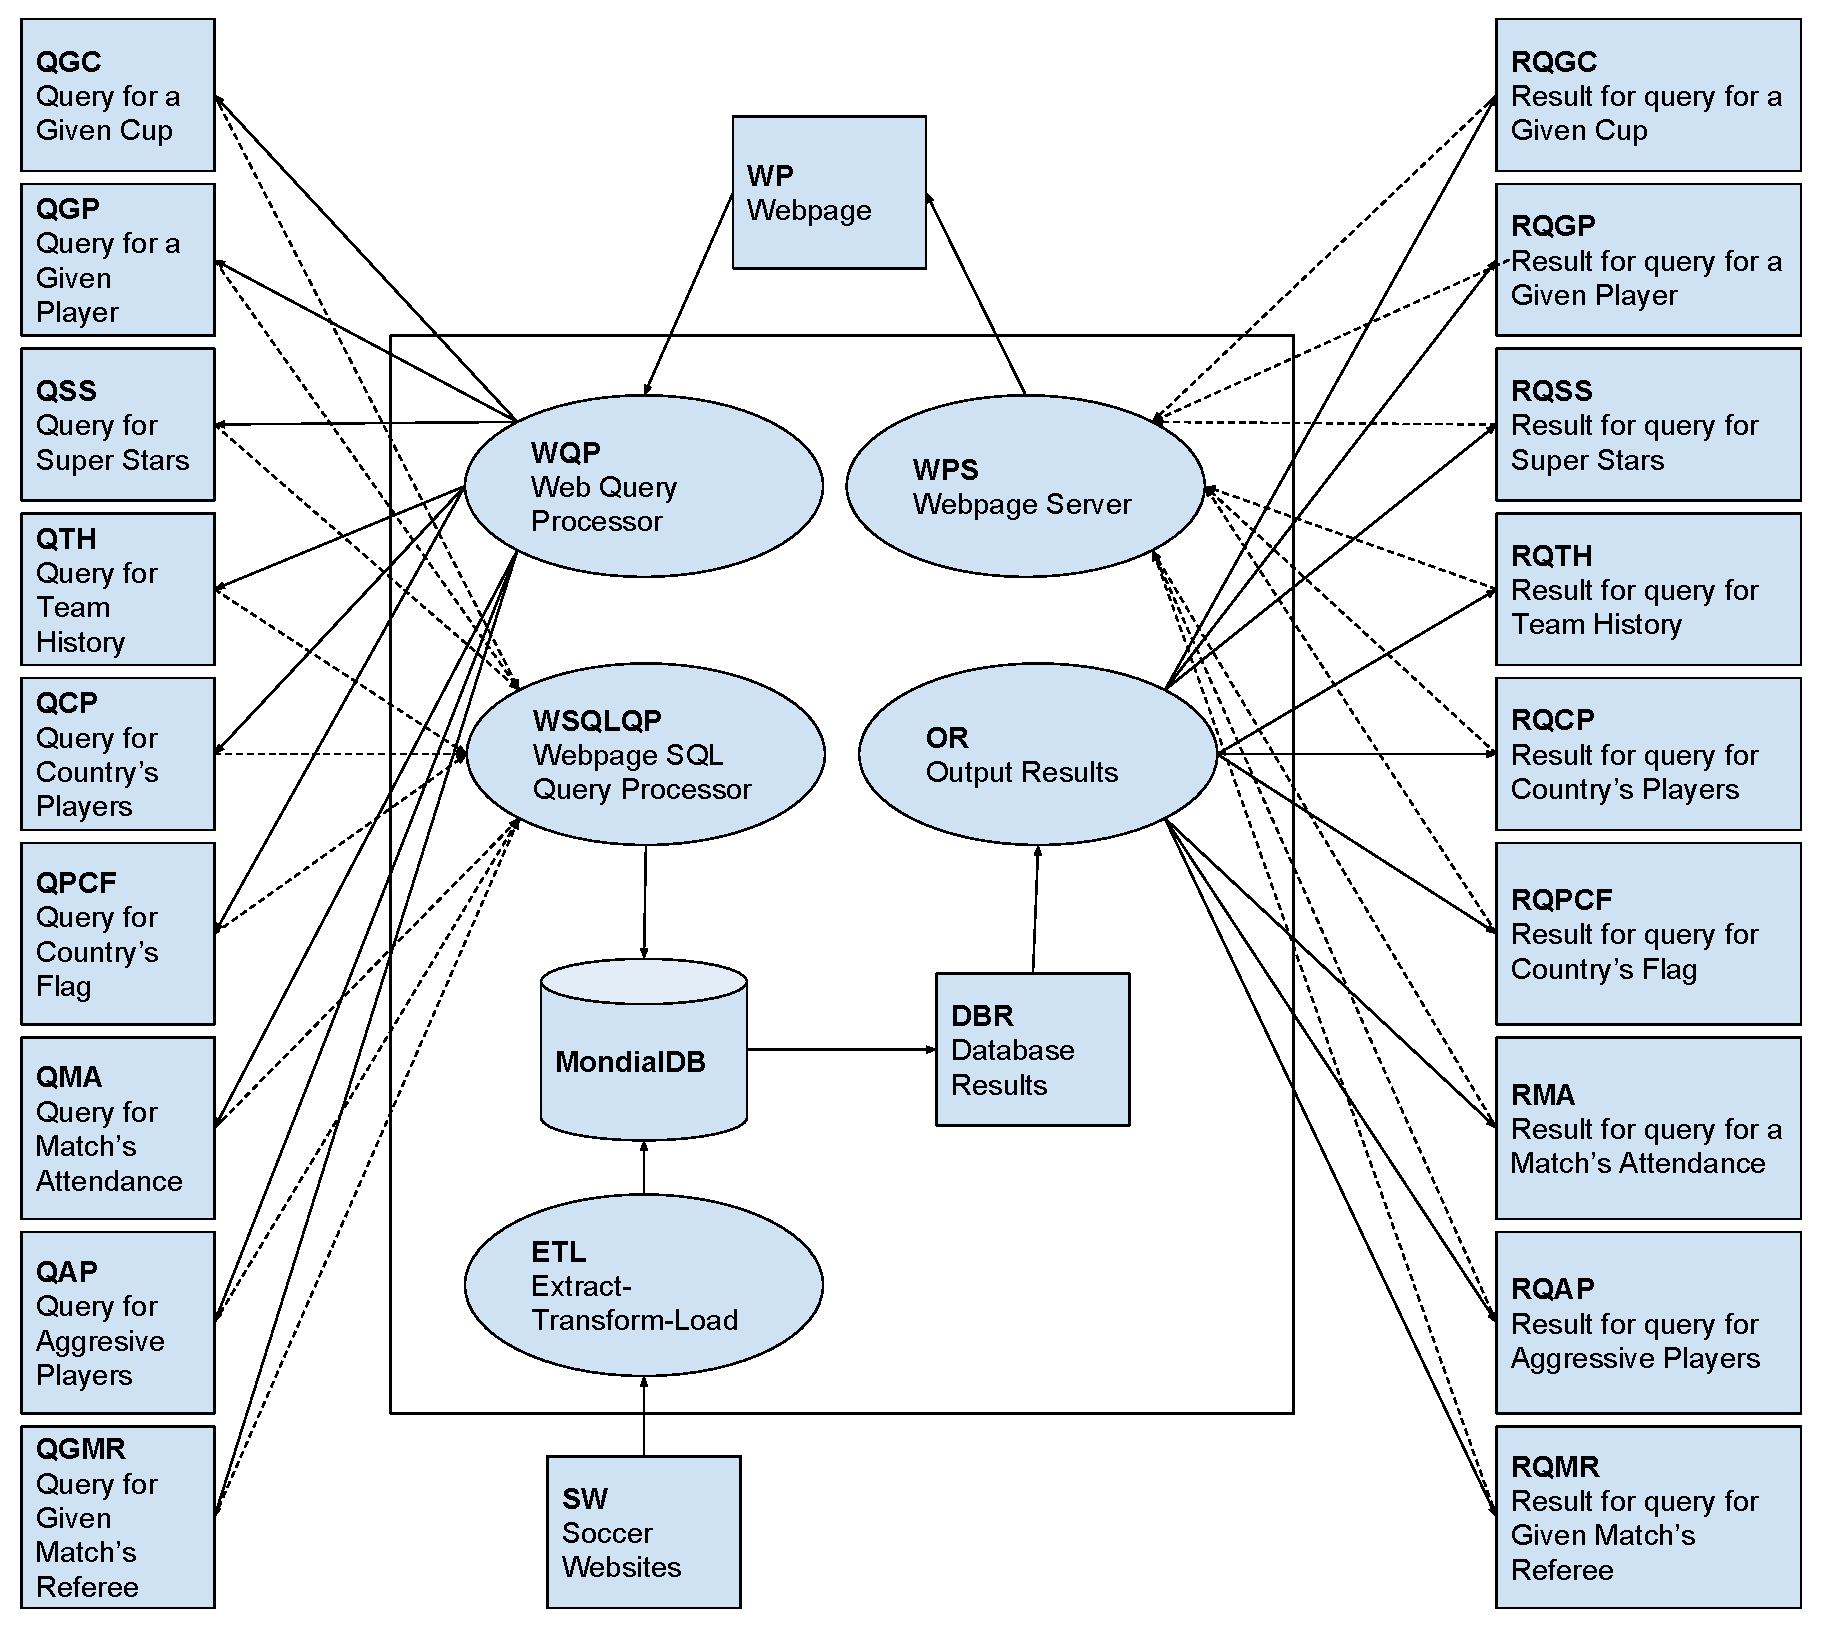
\includegraphics[height=462pt, angle=90]{dbflowdiagram}
\caption{Information Flow Diagram}
\label{flow}
\end{figure}

\clearpage

%\section{System Analysis and Specification}
\section{List of Tasks and Task Flow Diagram}
We describe the tasks and subtasks necessary to make, populate, and query MondialDB. 
See Figure~\ref{taskflow} on page \pageref{taskflow} for the Task Flow Diagram. 
The tasks are the following:
\begin{itemize}
  \item Extract, Transform, and Load Task
  \item Webpage Server Task
  \item Web Query Processor
  \item Webpage SQL Query Processor
  \item Output Results Task
\end{itemize}

\begin{figure}[ph]
\centering{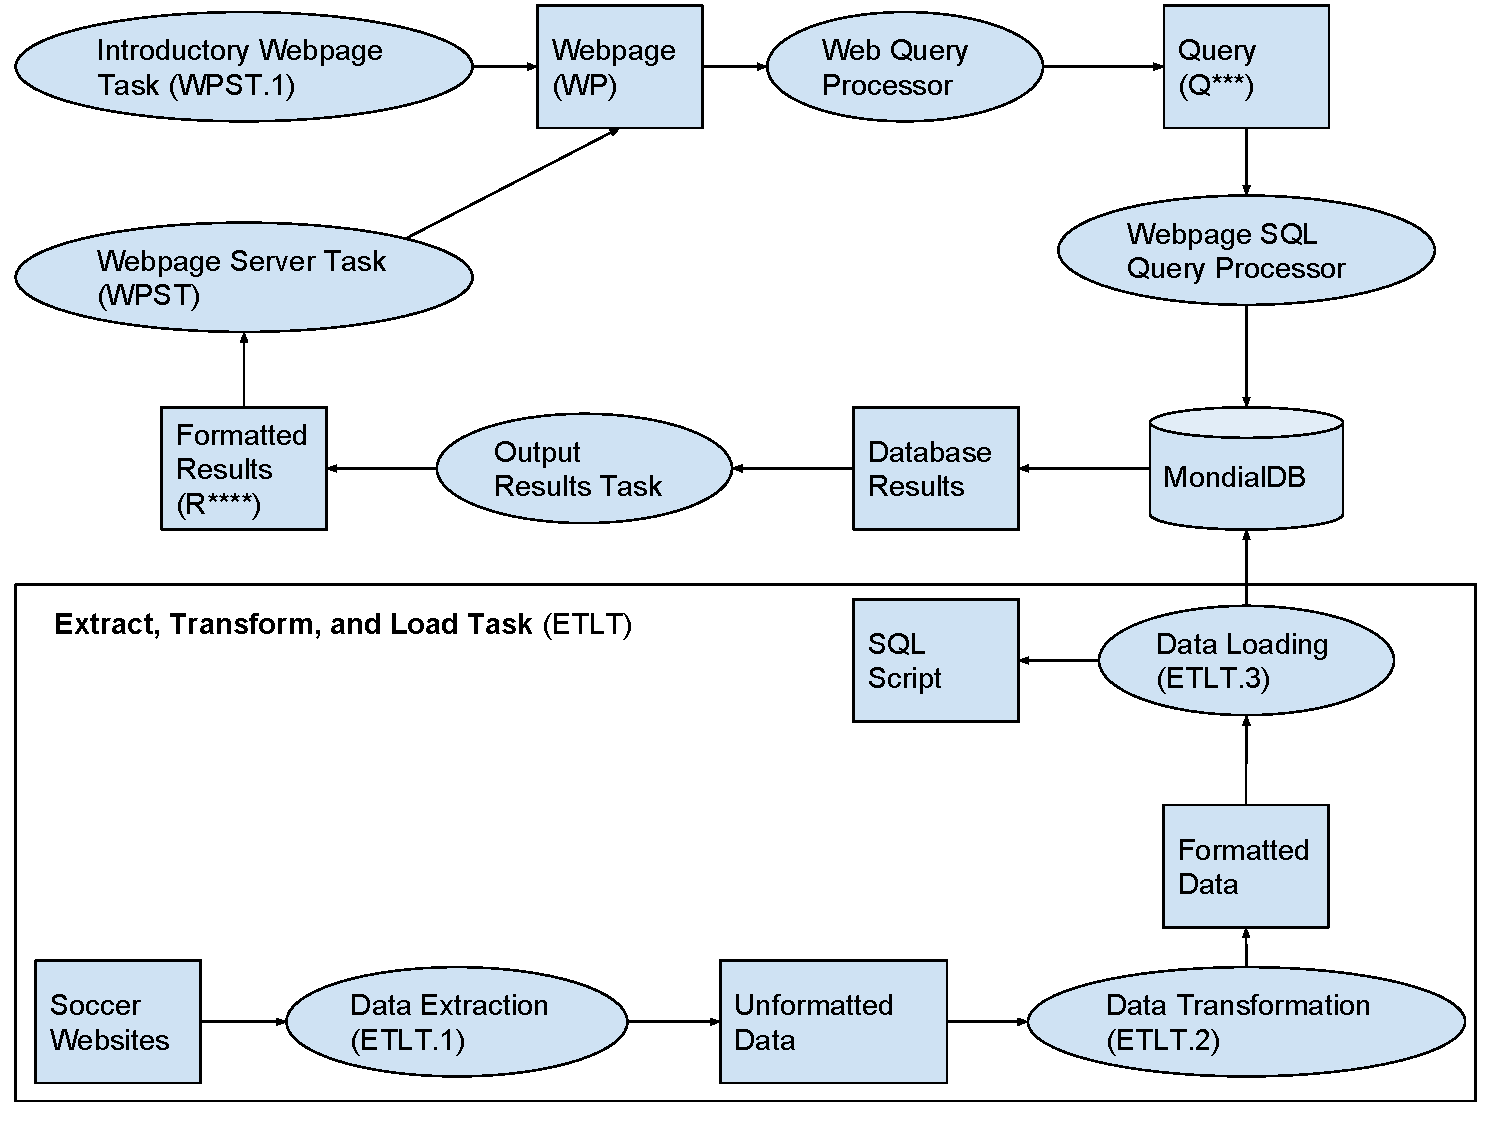
\includegraphics[width=\textwidth]{taskflowdiagram}}
\caption{Task Flow Diagram}
\label{taskflow}
\end{figure}

\clearpage

\subsection{Extract, Transform, and Load Task}
\begin{description}[noitemsep,align=right]
  \item[Task Label] ETLT
  \item[Task Name] Extract, Transform, and Load Task
  \item[Performer] Python script
  \item[Purpose] To extract data from Soccer Websites, transform it into a usable format, and send it to MondialDB
  \item[Enabling Condition] On database creation or database update
  \item[Description] It takes the information from Soccer Websites and puts the information into MondialDB.
  \item[Frequency] On database update
  \item[Duration] It will depend on the extraction, transformation, and load subtasks.
  \item[Importance] Most important
  \item[Maximum Delay] It depends on the subtasks.
  \item[Input] Soccer Websites
  \item[Output] Copy of the SQL script run by the python script as well as debugging information
  \item[Document Use] Soccer Websites, Unformatted Data, Formatted Data
  \item[Operations Performed] Data extraction, data transformation, and data loading
  \item[Subtasks] 
  Data extraction (ETLT.1), 
  data transformation (ETLT.2), 
  data loading (ETLT.3)  
  \item[Error Conditions] Errors from subtasks
\end{description}

\subsubsection{Data Extraction}
\begin{description}[noitemsep,align=right]
  \item[Task Label] ETLT.1
  \item[Task Name] Data Extraction
  \item[Performer] Python script
  \item[Purpose] To extract data from Soccer Websites
  \item[Enabling Condition] On database data insertion
  \item[Description] It pulls HTML from the Soccer Websites. 
  It then parses the HTML for data to put into MondialDB.  
  \item[Frequency] On database update
  \item[Duration] It depends on how quickly websites are scraped and extracted.
  \item[Importance] Most important
  \item[Maximum Delay] It depends on how many Soccer Websites are chosen.
  \item[Input] Soccer Websites
  \item[Output] Unformatted Data from the Soccer Websites
  \item[Document Use] Soccer Websites -\textgreater{} Unformatted Data
  \item[Operations Performed] Data extraction
  \item[Subtasks] None
  \item[Error Conditions] Soccer Websites are invalid. The format of the website is invalid or confusing.
\end{description}


\newpage

\subsubsection{Data Transformation}
\begin{description}[noitemsep,align=right]
  \item[Task Label] ETLT.2
  \item[Task Name] Data Transformation
  \item[Performer] Python script
  \item[Purpose] To transform data from Soccer Websites into a standardized format
  \item[Enabling Condition] On database data insertion
  \item[Description] It standardizes the data produced by Data Extraction. For example, names that are formatted like "Last Name, First Name" and "First Name Last Name" shall be changed into a standard format.
  \item[Frequency] On database update
  \item[Duration] It depends on how quickly the data goes from being unformatted to being formatted.
  \item[Importance] Important
  \item[Maximum Delay] It depends on how badly the original data was formatted.
  \item[Input] Unformatted Data from Data Extraction
  \item[Output] Formatted Data 
  \item[Document Use] Unformatted Data -\textgreater{} Formatted Data
  \item[Operations Performed] Data transformation
  \item[Subtasks] None
  \item[Error Conditions] The data are formatted badly.
\end{description}

\subsubsection{Data Loading}
\begin{description}[noitemsep,align=right]
  \item[Task Label] ETLT.3
  \item[Task Name] Data Loading
  \item[Performer] Python script
  \item[Purpose] To load formatted data into MondialDB
  \item[Enabling Condition] On database data insertion
  \item[Description] Makes an SQL script that inserts the standardized data from Data Transformation into MondialDB.
  \item[Frequency] On database update
  \item[Duration] It depends on how quickly the data is inserted into MondialDB
  \item[Importance] Most important
  \item[Maximum Delay]  It depends on how the slow the connection between the data collector and the database is.
  \item[Input] Formatted Data
  \item[Output] Log from inserting into MondialDB. Copy of the SQL script run by the python script.
  \item[Document Use] Formatted Data -\textgreater{} SQL Script
  \item[Operations Performed] Data Loading
  \item[Subtasks] None
  \item[Error Conditions] There is a faulty connection with the database.
\end{description}

\newpage

\subsection{Web Query Processor}
\begin{description}[noitemsep,align=right]
  \item[Task Label] WQPT
  \item[Task Name] Web Query Processor
  \item[Performer] Web-server
  \item[Purpose] Processes queries from the web-server and sends the respective query to the Webpage SQL Query Processor Task. 
  \item[Enabling Condition] After web-server runs
  \item[Description] It determines the user-specified query from the forms on the Webpage. Once this query is validated, it sends the query on to the Webpage SQL Query Processor.
  \item[Frequency]  Always on
  \item[Duration] As long as the database is active
  \item[Importance] Important
  \item[Maximum Delay] Response delay to user requests should be short and less than 10 seconds.
  \item[Input] User-inputted form data from the Webpage
  \item[Output] Sends Query type to Webpage SQL Processor Task. See Query Types.
  \item[Document Use] Webpage -\textgreater{} Query
  \item[Operations Performed] Validates queries and determines query type.
  \item[Subtasks] None
  \item[Error Conditions] The query isn't valid.
\end{description}

\newpage

\subsection{Webpage SQL Query Processor Task}
\begin{description}[noitemsep,align=right]
  \item[Task Label] WSQLQPT
  \item[Task Name] Webpage SQL Query Processor Task
  \item[Performer] Webpage server
  \item[Purpose] Sends the query from the user-specified query task to MondialDB
  \item[Enabling Condition] User submits valid query
  \item[Description] The WSQLQPT is the final step before the query reaches MondialDB. It will send a perform a raw SQL query in MondialDB
  \item[Frequency]  Triggers on every received valid user query
  \item[Duration] The SQL shouldn't take longer than 15 seconds to run.
  \item[Importance] Important 
  \item[Maximum Delay] The SQL shouldn't take at most longer than 45 seconds to run.
  \item[Input] User-specified query from the following list:

    QGC (Query for a given cup)
    
    QGP (Query for a given player)
    
    QSS(Query for Super Stars)
    
    QTH(Query for Team History)
    
    QCP(Query for Country's Players)
    
    QPCF(Query for Country's Flag)
    
    QMA (Query for Match's Attendance)
    
  	QAP (Query for Aggressive Players)
    
    QGMR (Query for a Given Match's Referee)
    
  \item[Output] Sends SQL query to MondialDB
  \item[Document Use] Query  
  \item[Operations Performed]  If the query is a valid query from the aforementioned list, then create the SQL command. If it is not a valid query, send an error message back.
  \item[Subtasks] None
  \item[Error Conditions] The user-specified query is not valid.  
\end{description}

\newpage

\subsection{Output Results Task}
\begin{description}[noitemsep,align=right]
  \item[Task Label] OR
  \item[Task Name] Output Results Task
  \item[Performer] Webpage Server
  \item[Purpose] Sends the query results to the user
  \item[Enabling Condition] MondialDB receives query and sends output to Output Results Task
  \item[Description] The WSQLQPT is the final step before the query reaches MondialDB. It will send a raw SQL query to MondialDB.
  \item[Frequency]  Triggers on every received request
  \item[Duration] In ideal network conditions, it should be short and less than 10 seconds.
  \item[Importance] Most Important
  \item[Maximum Delay] Response delay to user requests should be short and less than 10 seconds.
  \item[Input] For a user-specified query, Database Results
  \item[Output] The Formatted Result from the results  
  \item[Document Use] Database Results -\textgreater{} Formatted Results
  \item[Operations Performed] Sends query results to Webpage Server Task 
  \item[Subtasks] None
  \item[Error Conditions] MondialDB gave back error conditions instead of valid results. Connection to user is disrupted. Web server becomes overloaded.
\end{description}

\newpage

\section{List of Documents}
See page \pageref{taskflow2} for repeated Task Flow Diagram. The documents are the following:
\begin{itemize}
	\item Webpage
	\item Query 
	\item Database Results
	\item Formatted Results
	\item Soccer Websites
	\item Unformatted Data
	\item Formatted Data
	\item SQL Script
\end{itemize}

\begin{figure}[ph]
	\centering{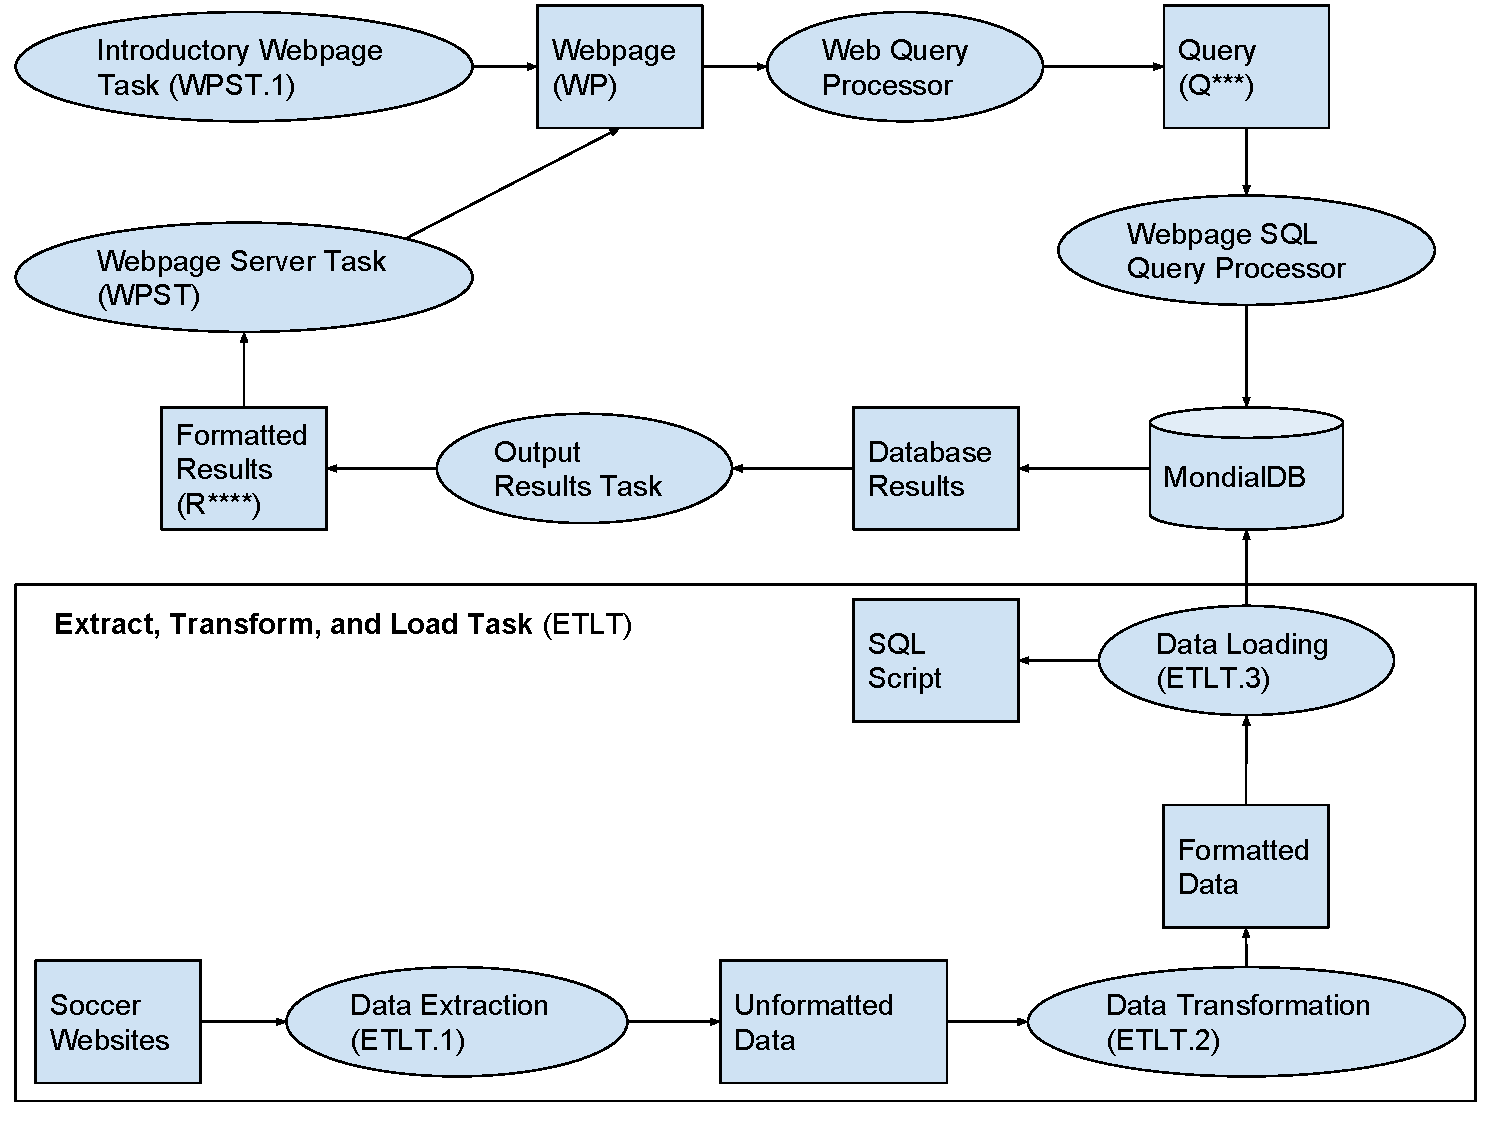
\includegraphics[width=\textwidth]{taskflowdiagram}}
	\caption{Task Flow Diagram}
	\label{taskflow2}
\end{figure}

\subsection{Queries}
The types of Queries:
\begin{itemize}
	\label{queries}
	\item QGC (Query for a given cup)
	\item QGP (Query for a given player)
	\item QSS (Query for Super Stars)
	\item QTH (Query for Team History)
	\item QCP (Query for Country's Players)
	\item QPCF(Query for Country's Flag)
	\item QMA (Query for Match's Attendance)
	\item QGMS (Query for Aggressive Players)
	\item QGMR (Query for a Given Match's Referee)
\end{itemize}

\paragraph{Query for Country's Flag}
This query returns information about a country's flag. Most notably this includes a link to a picture of that country's flag. The query is interesting because it adds an extra dimension to the database. Users might find it easier
to recognize a country by its flag instead of by its name. Others might be curious and be inspired to learn more interesting information about flags.
Flags traditionally represent countries. They are symbols for the people of that country to rally around and to represent. They represent the history of the nation. Thus, they are interesting.
\paragraph{Query for Match's Attendance}
This query returns information about a specific match. It will give back what stadium the match was held in. It will also tell the user how many people attended that particular match. Attendance information is wonderfully informative. The user could try to find out what teams are most popular, what stadiums are most popular, or what host countries are most popular.  
\paragraph{Query for Aggressive Players}
This query tells users who the most aggressive players are. The metric of aggressiveness is determined by how many penalties they accumulate. It is interesting to see the human side of soccer and how vicious it can get.
\paragraph{Query for a Given Match's Referee}
This query tells users what referee was calling for a particular match. Many people assume referees are biased against the team that they like. By using this query, they could see if the referee really is biased against their favorite team.

\part{Phase 2 Documentation}

\section{ER Model}
\begin{figure}[ph]
	\centering{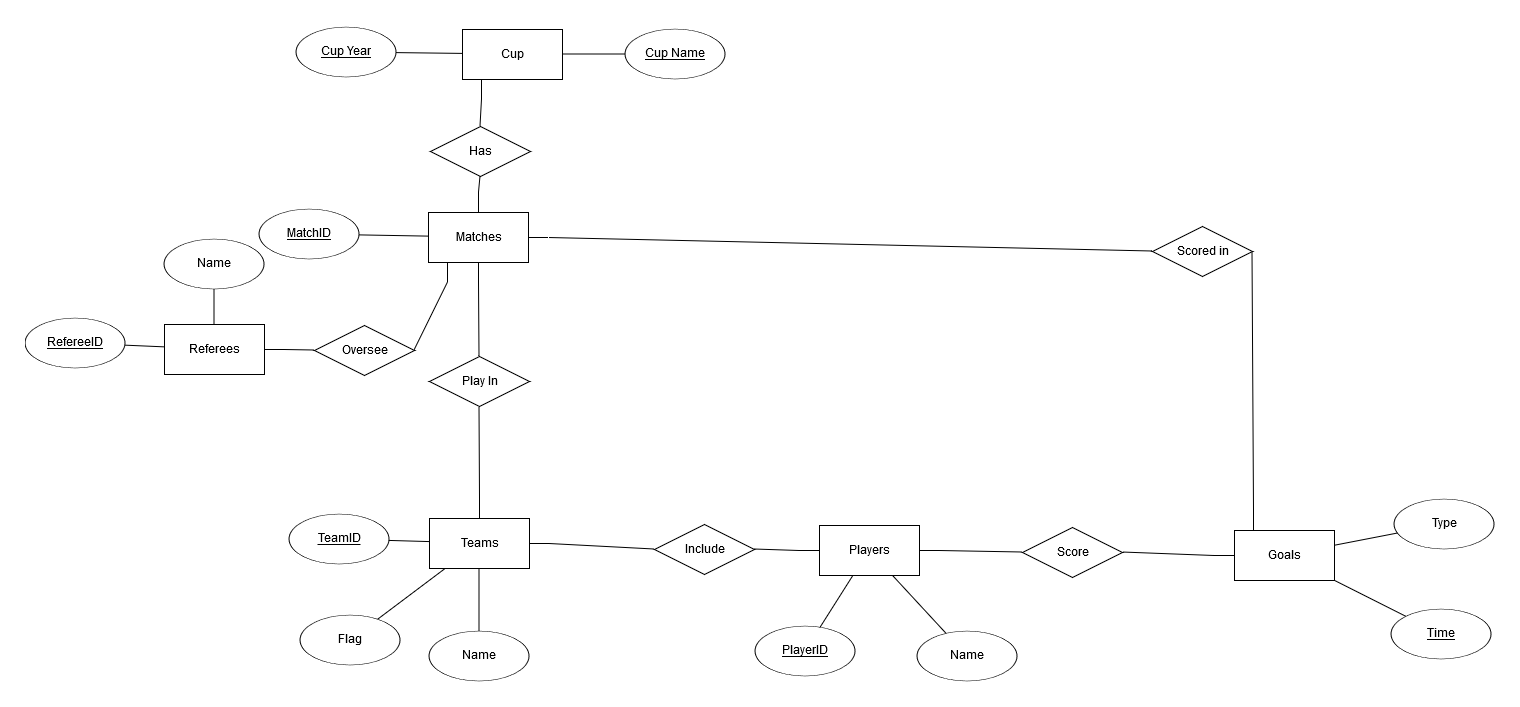
\includegraphics[width=\textwidth]{ermodel}}
	\caption {ER Model}
	\label{ermodel}
\end{figure}

\section{Relational Schema}
\begin{figure}[ph]
	\centering{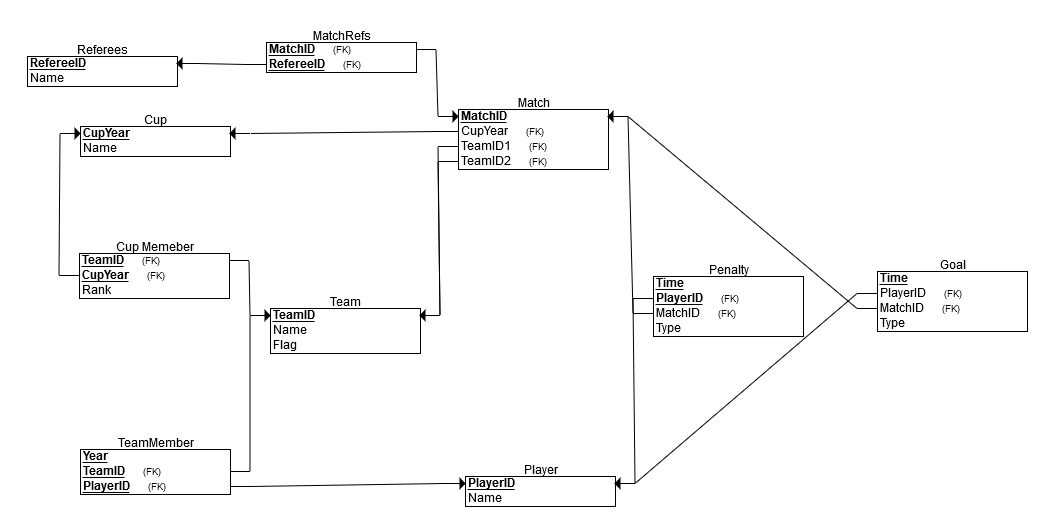
\includegraphics[width=\textwidth]{relschema}}
	\caption{Relational Schema}
	\label{relschema}
\end{figure}

\section{Query for Super Stars}
\begin{lstlisting}[language=SQL]
--Get super stars
CREATE VIEW super_stars AS
SELECT tm1.playerID,cm.CupYear
FROM CupMember cm, TeamMember tm1, TeamMember tm2.
WHERE tm1.playerID==tm2.playerID
AND tm1.year!=tm2.year
AND cm.TeamID=tm1.teamID
\end{lstlisting}

\newpage

\section{Query for a Given Player}
\begin{lstlisting}[language=SQL]
--Players with said name
CREATE VIEW player_ids AS
SELECT p.playerID
FROM player p
WHERE p.name=selected_name

--Teams those players were on
CREATE VIEW team_ids AS
SELECT tm.teamID, pids.playerID
FROM TeamMember tm,player_ids pids
WHERE tm.playerID=pids.p

--Team Names
SELECT t.name
FROM team_ids tids, team t
WHERE t.teamID=tids.teamID

--Cups those players were in
CREATE VIEW cup_years AS
SELECT cm.CupYear, tid.PlayerID
FROM CupMember cm, team_ids tids
WHERE cm.teamID=            tids.TeamID

--Regular Goals
SELECT g.playerID, count(g.playerID)
FROM Goal g, player_ids pids
WHERE g.type=’Regular’ and g.PlayerID==pid.playerId
GROUP BY g.playerID

--Penalty shots
SELECT g.playerID, count(g.playerID)
FROM Goal g, player_ids pids
WHERE g.type=’Penalty’ and g.PlayerID==pid.playerId
GROUP BY g.playerID
\end{lstlisting}

\newpage

\section{Query for Team History}
\begin{lstlisting}[language=SQL]
SELECT c.name, c.year, t1.name, t2.name
FROM  cup c. team t2,match m
WHERE m.cupyear=c.cupyear
AND m.teamID1=t1.teamID
AND m.teamID2=t2.teamID

SELECT c.Name,t.name , cm.cupyear, cm.rank
FROM team t, cupmember cm, cup c
WHERE t.teamId=cm.teamId
AND c.cupyear=cm.cupyear

SELECT p.name,m.name,p.time,p.type
FROM penalty p, match m,player pl
WHERE m.matchID=p.matchID
AND p1.playerID=p.playerID
\end{lstlisting}

\section{Query for a given Cup}
\begin{lstlisting}[language=SQL]
--Teams
CREATE VIEW participating_team_ids AS
SELECT cm.teamID
FROM CupMember cm
WHERE cm.CupYear=SelectedYear;

--Ranks
SELECT t.name, cm.rank
FROM participating_team_ids ids, CupMember cm,Team t
WHERE ids.teamID==t.TeamID
AND ids.teamID==cm.teamID
AND cm.CupYear=selected year

--Regular Goals
SELECT g.matchID, count(g.time)
FROM Goal g, match m
WHERE g.type=’Regular’ and g.matchID==m.matchID
GROUP BY g.matchID

--Penalty shots
SELECT g.matchID, count(g.time)
FROM Goal g, match m
WHERE g.type=’Penalty’ and g.matchID==m.matchID
GROUP BY g.matchID
\end{lstlisting}
\newpage

\section{Pseudo code for Extract and Transform Task}
The pseudo code for extracting can be thoroughly extended.
The basic process is to grab the html of a website, parse it, and then execute a regex on its contents to capture data. The following is a code snippet:
\lstinputlisting[language=Python]{extractphase2.py}

\newpage
\section{Pseudo code For Load Task}
The following is a code snippet:
\lstinputlisting[language=Python]{loadphase2.py}


\end{document}  